\section{PBMPM 参数调参补充分析}

本节使用 PBMPM 调参包中的 $21$ 组 run 分析 \texttt{pbmpm\_elastic\_relaxation} 和 \texttt{pbmpm\_strength\_scale} 的作用。其中 $20$ 组成功完成，$1$ 组失败；所有 run 的 NaN 数和 Inf 数均为 $0$。当前数据中的 projection residual 和 constraint residual 字段为空，因此本节不据此评价约束误差，而主要依据成功状态、耗时、motion、bbox 和渲染结果判断。

离线渲染包中的相机移动未关闭，因此本节插图会有轻微视角旋转；视觉判断主要用于辅助辨认形变幅度和过度弯曲现象。

\subsection{relaxation=1.5 下的通用表现}

首先固定 $s_{\mathrm{str}}=1.0$、$\omega=1.5$。网格消融结果见表~\ref{tab:pbmpm-common-grid-rel15}。
\begin{table}[H]
\centering
\caption{PBMPM 在 $\omega=1.5$ 下的网格消融}
\label{tab:pbmpm-common-grid-rel15}
\small
\resizebox{\textwidth}{!}{%
\begin{tabular}{lccccccccc}
\toprule
$n_{\mathrm{grid}}$ & 成功 & 内步/理论 & 投影迭代 & 耗时/s & $d_{\max}$ & $\bar d$ & $v_{\max}$ & $a_{\max}$ & $r_{\mathrm{bbox}}$ \\
\midrule
$25$ & 是 & 6000/6000 & 3.0 & 40.65 & 0.0051 & 0.0008 & 0.257 & 15.72 & 1.0005 \\
$50$ & 是 & 6000/6000 & 5.0 & 46.88 & 0.0356 & 0.0023 & 1.208 & 37.17 & 1.0016 \\
$100$ & 是 & 6000/6000 & 11.00 & 75.91 & 0.1625 & 0.0154 & 3.680 & 76.12 & 1.0218 \\
\bottomrule
\end{tabular}%
}
\end{table}
\begin{figure}[H]
    \centering
    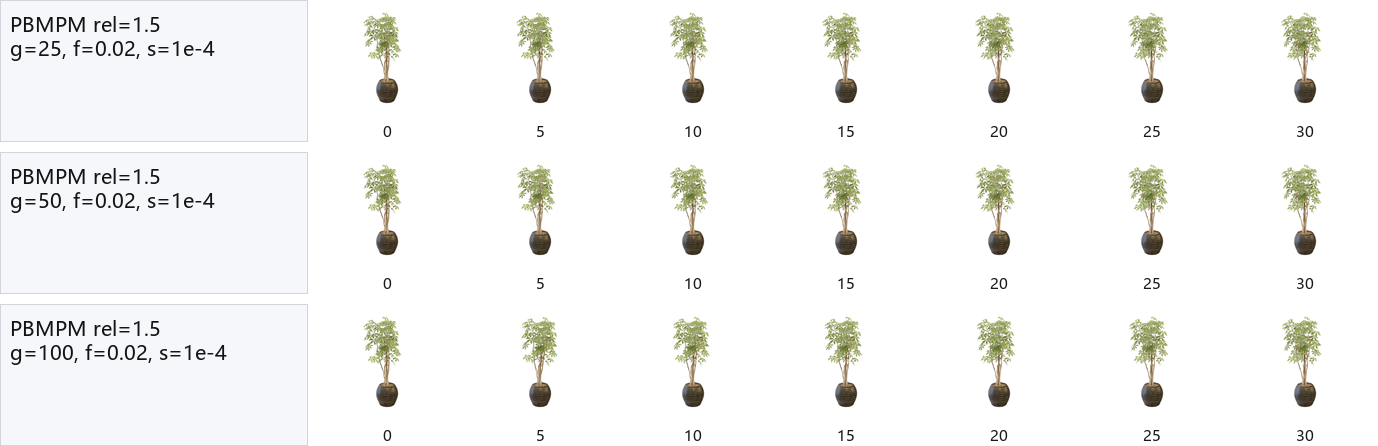
\includegraphics[width=\textwidth,height=0.31\textheight,keepaspectratio]{figures/render_strips/group_pbmpm_eval_common_grid.png}
    \caption{PBMPM 在 $\omega=1.5$ 下的网格消融渲染关键帧。每行从左到右为第 $0,5,10,15,20,25,30$ 帧。}
    \label{fig:pbmpm-eval-common-grid}
\end{figure}
\FloatBarrier
可以看到，$n_{\mathrm{grid}}=100$ 时投影迭代次数增至 $11$，最大位移、速度和加速度均明显高于 $25$ 与 $50$。这说明 relaxation 解耦后，细网格下 PBMPM 仍会放大 motion；视觉上树体弯曲也更明显。

子步长消融结果见表~\ref{tab:pbmpm-common-substep-rel15}。
\begin{table}[H]
\centering
\caption{PBMPM 在 $\omega=1.5$ 下的子步长消融}
\label{tab:pbmpm-common-substep-rel15}
\small
\resizebox{\textwidth}{!}{%
\begin{tabular}{lccccccccc}
\toprule
$\Delta t_{\mathrm{sub}}$ & 成功 & 内步/理论 & 投影迭代 & 耗时/s & $d_{\max}$ & $\bar d$ & $v_{\max}$ & $a_{\max}$ & $r_{\mathrm{bbox}}$ \\
\midrule
$10^{-4}$ & 是 & 6000/6000 & 5.0 & 46.88 & 0.0356 & 0.0023 & 1.208 & 37.17 & 1.0016 \\
$5\times10^{-4}$ & 是 & 1200/1200 & 24.00 & 38.66 & 0.4417 & 0.0070 & 7.568 & 133.9 & 1.0071 \\
$10^{-3}$ & 是 & 600/600 & 24.00 & 22.42 & 1.6493 & 0.2556 & 16.11 & 313.2 & 1.2151 \\
\bottomrule
\end{tabular}%
}
\end{table}
\begin{figure}[H]
    \centering
    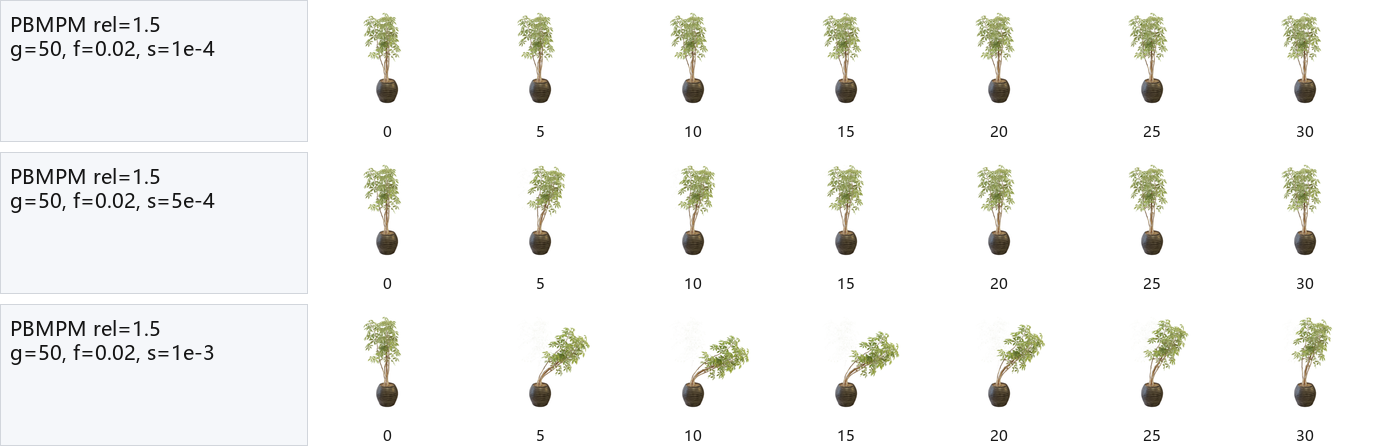
\includegraphics[width=\textwidth,height=0.31\textheight,keepaspectratio]{figures/render_strips/group_pbmpm_eval_common_substep.png}
    \caption{PBMPM 在 $\omega=1.5$ 下的子步长消融渲染关键帧。}
    \label{fig:pbmpm-eval-common-substep}
\end{figure}
\FloatBarrier
$\Delta t_{\mathrm{sub}}=10^{-3}$ 虽然成功完成，但最大位移达到 $1.6493$，bbox 体积比达到 $1.2151$，图中树体已经出现明显过度弯曲。因此 PBMPM 的 success 只说明程序生成了 motion，不等价于 motion 合理。

\subsection{relaxation 参数实验}

在 $n_{\mathrm{grid}}=100$ 下扫描 $\omega$，结果见表~\ref{tab:pbmpm-relax-grid100}。
\begin{table}[H]
\centering
\caption{PBMPM 在 $n_{\mathrm{grid}}=100$ 下的 relaxation 实验}
\label{tab:pbmpm-relax-grid100}
\small
\resizebox{\textwidth}{!}{%
\begin{tabular}{lccccccccc}
\toprule
$\omega$ & 成功 & 内步/理论 & 投影迭代 & 耗时/s & $d_{\max}$ & $\bar d$ & $v_{\max}$ & $a_{\max}$ & $r_{\mathrm{bbox}}$ \\
\midrule
$0.0$ & 是 & 6000/6000 & 11.00 & 77.44 & 0.3387 & 0.1998 & 4.173 & 66.54 & 1.0647 \\
$1.0$ & 是 & 6000/6000 & 11.00 & 75.50 & 0.1725 & 0.0255 & 3.695 & 70.87 & 1.0267 \\
$1.5$ & 是 & 6000/6000 & 11.00 & 75.91 & 0.1625 & 0.0154 & 3.680 & 76.12 & 1.0218 \\
$2.0$ & 是 & 6000/6000 & 11.00 & 75.93 & 0.1546 & 0.0107 & 3.669 & 79.87 & 1.0187 \\
\bottomrule
\end{tabular}%
}
\end{table}
\begin{figure}[H]
    \centering
    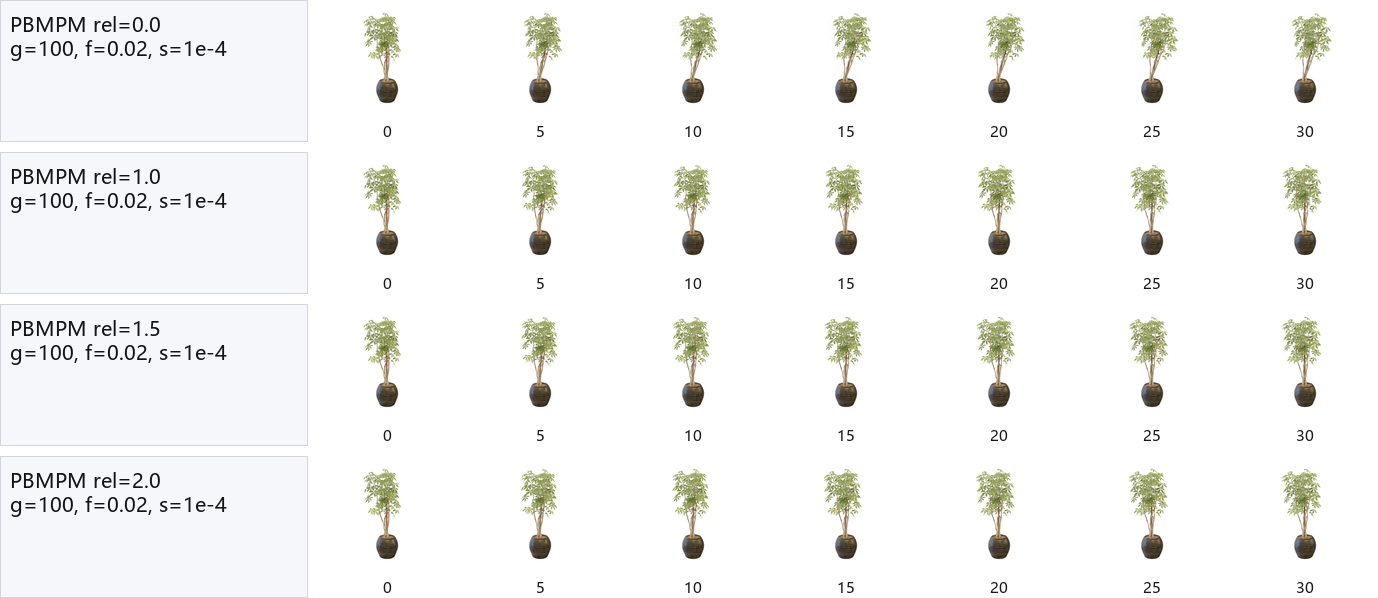
\includegraphics[width=\textwidth,height=0.40\textheight,keepaspectratio]{figures/render_strips/group_pbmpm_eval_relax_grid100.png}
    \caption{PBMPM 在 $n_{\mathrm{grid}}=100$ 下扫描 relaxation 的渲染关键帧。}
    \label{fig:pbmpm-eval-relax-grid100}
\end{figure}
\FloatBarrier
随着 $\omega$ 从 $0$ 增大到 $2$，平均位移从 $0.1998$ 降至 $0.0107$，bbox 体积比从 $1.0647$ 降至 $1.0187$；但最大加速度从 $66.54$ 升至 $79.87$。这说明 relaxation 是关键稳定参数，但较强投影也可能带来更尖锐的局部速度变化。

在 $\Delta t_{\mathrm{sub}}=10^{-3}$ 下扫描 $\omega$，结果见表~\ref{tab:pbmpm-relax-dt001}。
\begin{table}[H]
\centering
\caption{PBMPM 在 $\Delta t_{\mathrm{sub}}=10^{-3}$ 下的 relaxation 实验}
\label{tab:pbmpm-relax-dt001}
\small
\resizebox{\textwidth}{!}{%
\begin{tabular}{lccccccccc}
\toprule
$\omega$ & 成功 & 内步/理论 & 投影迭代 & 耗时/s & $d_{\max}$ & $\bar d$ & $v_{\max}$ & $a_{\max}$ & $r_{\mathrm{bbox}}$ \\
\midrule
$0.0$ & 否 & 137/600 & 24.00 & 10.57 & 1.6918 & 1.0298 & 17.98 & 151.0 & 2.4005 \\
$1.0$ & 是 & 600/600 & 24.00 & 22.78 & 1.6811 & 0.3767 & 16.22 & 281.6 & 1.3003 \\
$1.5$ & 是 & 600/600 & 24.00 & 22.42 & 1.6493 & 0.2556 & 16.11 & 313.2 & 1.2151 \\
$2.0$ & 是 & 600/600 & 24.00 & 22.80 & 1.5650 & 0.1281 & 16.03 & 329.7 & 1.0991 \\
\bottomrule
\end{tabular}%
}
\end{table}
\begin{figure}[H]
    \centering
    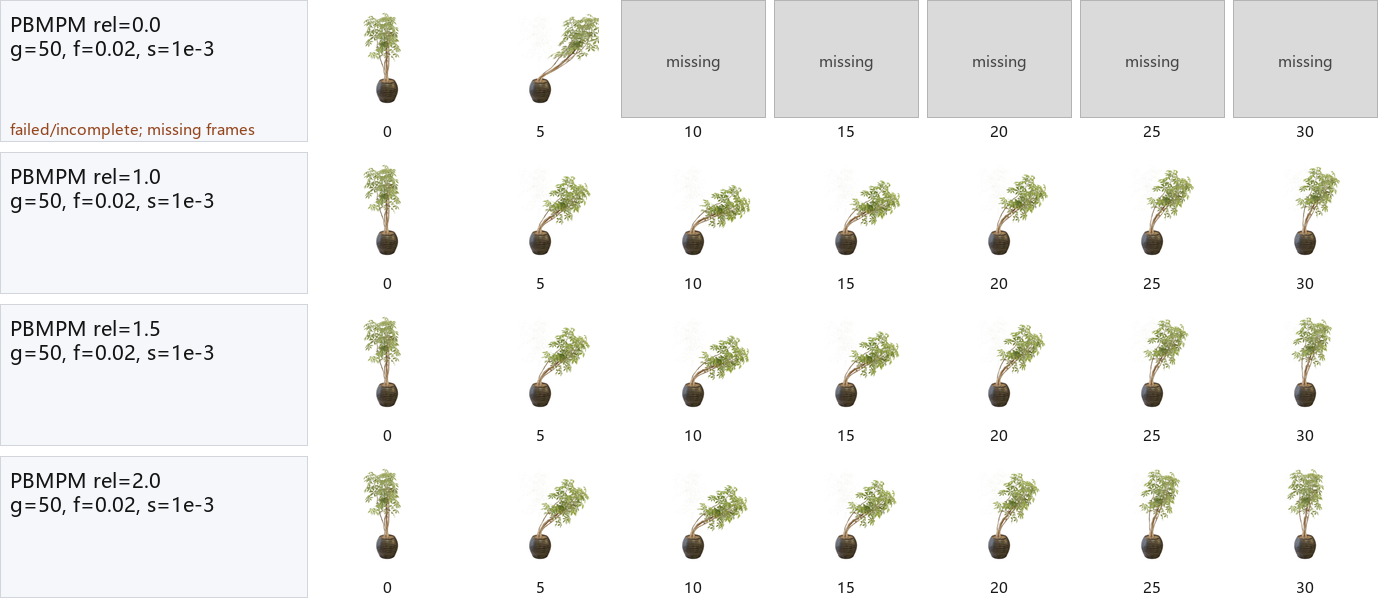
\includegraphics[width=\textwidth,height=0.40\textheight,keepaspectratio]{figures/render_strips/group_pbmpm_eval_relax_dt001.png}
    \caption{PBMPM 在 $\Delta t_{\mathrm{sub}}=10^{-3}$ 下扫描 relaxation 的渲染关键帧；缺失帧以灰色占位表示。}
    \label{fig:pbmpm-eval-relax-dt001}
\end{figure}
\FloatBarrier
$\omega=0$ 的 run 只生成 $7$ 帧并以 \texttt{exit\_code\_-6} 失败，$\omega=1,1.5,2$ 均能完成。增大 $\omega$ 可显著降低平均位移和 bbox 膨胀，但最大位移仍保持在 $1.5$ 以上，说明 relaxation 解耦改善了大时间步稳定性，却不能完全消除大时间步导致的 motion 放大。

\subsection{strength 参数实验}

在 $n_{\mathrm{grid}}=100$ 下扫描 strength，结果见表~\ref{tab:pbmpm-strength-grid100}。
\begin{table}[H]
\centering
\caption{PBMPM 在 $n_{\mathrm{grid}}=100$ 下的 strength 实验}
\label{tab:pbmpm-strength-grid100}
\small
\resizebox{\textwidth}{!}{%
\begin{tabular}{lccccccccc}
\toprule
$s_{\mathrm{str}}$ & 成功 & 内步/理论 & 投影迭代 & 耗时/s & $d_{\max}$ & $\bar d$ & $v_{\max}$ & $a_{\max}$ & $r_{\mathrm{bbox}}$ \\
\midrule
$0.25$ & 是 & 6000/6000 & 5.0 & 44.26 & 0.2650 & 0.0525 & 3.990 & 57.77 & 1.0419 \\
$0.50$ & 是 & 6000/6000 & 8.0 & 60.08 & 0.2008 & 0.0282 & 3.825 & 67.15 & 1.0307 \\
$1.00$ & 是 & 6000/6000 & 11.00 & 75.91 & 0.1625 & 0.0154 & 3.680 & 76.12 & 1.0218 \\
$2.00$ & 是 & 6000/6000 & 17.00 & 109.6 & 0.1213 & 0.0072 & 3.431 & 87.57 & 1.0133 \\
$4.00$ & 是 & 6000/6000 & 22.00 & 135.0 & 0.1000 & 0.0041 & 3.242 & 96.73 & 1.0086 \\
\bottomrule
\end{tabular}%
}
\end{table}
\begin{figure}[H]
    \centering
    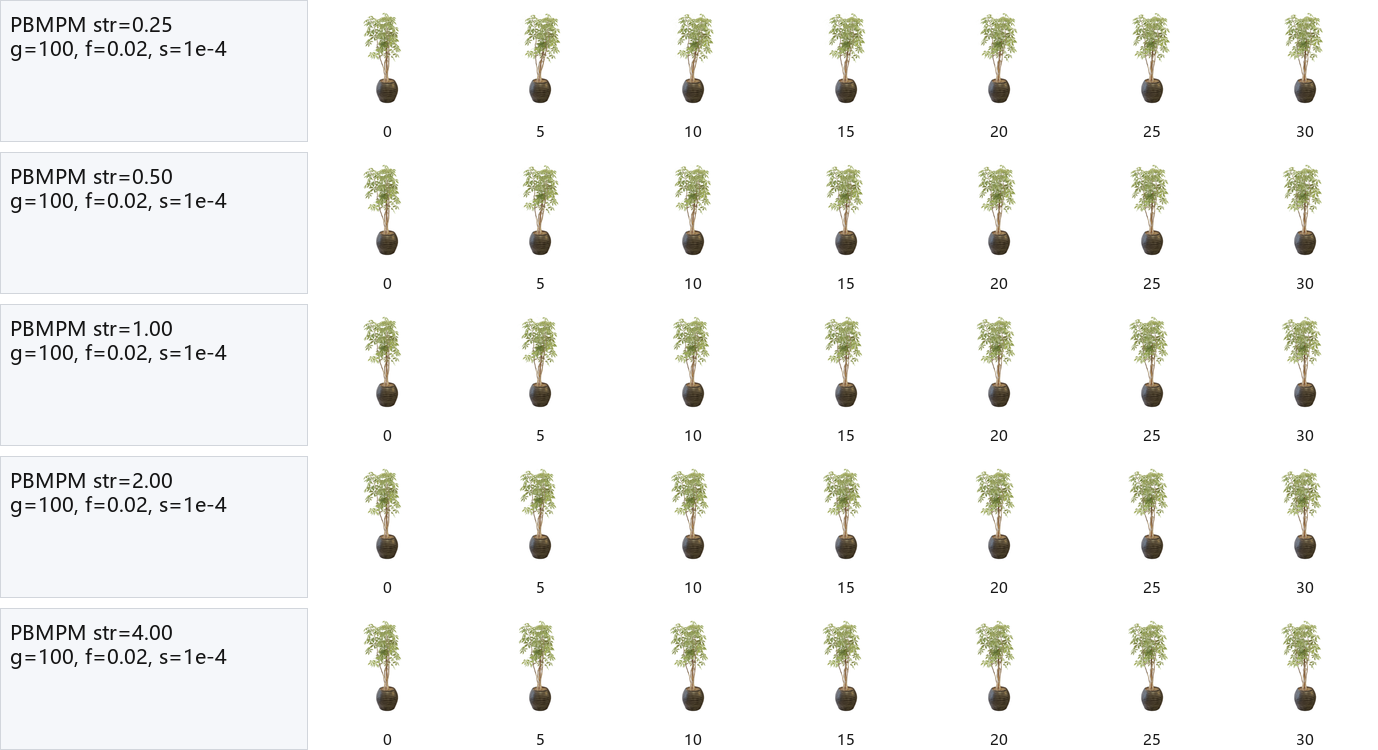
\includegraphics[width=\textwidth,height=0.45\textheight,keepaspectratio]{figures/render_strips/group_pbmpm_eval_strength_grid100.png}
    \caption{PBMPM 在 $n_{\mathrm{grid}}=100$ 下扫描 strength 的渲染关键帧。}
    \label{fig:pbmpm-eval-strength-grid100}
\end{figure}
\FloatBarrier
strength 从 $0.25$ 增大到 $4.0$ 时，投影迭代次数从 $5$ 增至 $22$，平均位移从 $0.0525$ 降至 $0.0041$，bbox 体积比从 $1.0419$ 降至 $1.0086$。因此在细网格设置下，strength 对约束强度和形变幅度有明显作用；同时最大加速度随 strength 增大而升高，说明更强投影会提高局部运动尖峰风险。

在 $\Delta t_{\mathrm{sub}}=10^{-3}$ 下扫描 strength，结果见表~\ref{tab:pbmpm-strength-dt001}。
\begin{table}[H]
\centering
\caption{PBMPM 在 $\Delta t_{\mathrm{sub}}=10^{-3}$ 下的 strength 实验}
\label{tab:pbmpm-strength-dt001}
\small
\resizebox{\textwidth}{!}{%
\begin{tabular}{lccccccccc}
\toprule
$s_{\mathrm{str}}$ & 成功 & 内步/理论 & 投影迭代 & 耗时/s & $d_{\max}$ & $\bar d$ & $v_{\max}$ & $a_{\max}$ & $r_{\mathrm{bbox}}$ \\
\midrule
$0.25$ & 是 & 600/600 & 24.00 & 22.56 & 1.6696 & 0.3001 & 16.15 & 303.4 & 1.2472 \\
$0.50$ & 是 & 600/600 & 24.00 & 22.49 & 1.6545 & 0.2648 & 16.11 & 311.4 & 1.2225 \\
$1.00$ & 是 & 600/600 & 24.00 & 22.42 & 1.6493 & 0.2556 & 16.11 & 313.2 & 1.2151 \\
$2.00$ & 是 & 600/600 & 24.00 & 22.74 & 1.6490 & 0.2551 & 16.10 & 313.3 & 1.2148 \\
$4.00$ & 是 & 600/600 & 25.00 & 23.05 & 1.6290 & 0.2443 & 16.08 & 315.5 & 1.2042 \\
\bottomrule
\end{tabular}%
}
\end{table}
\begin{figure}[H]
    \centering
    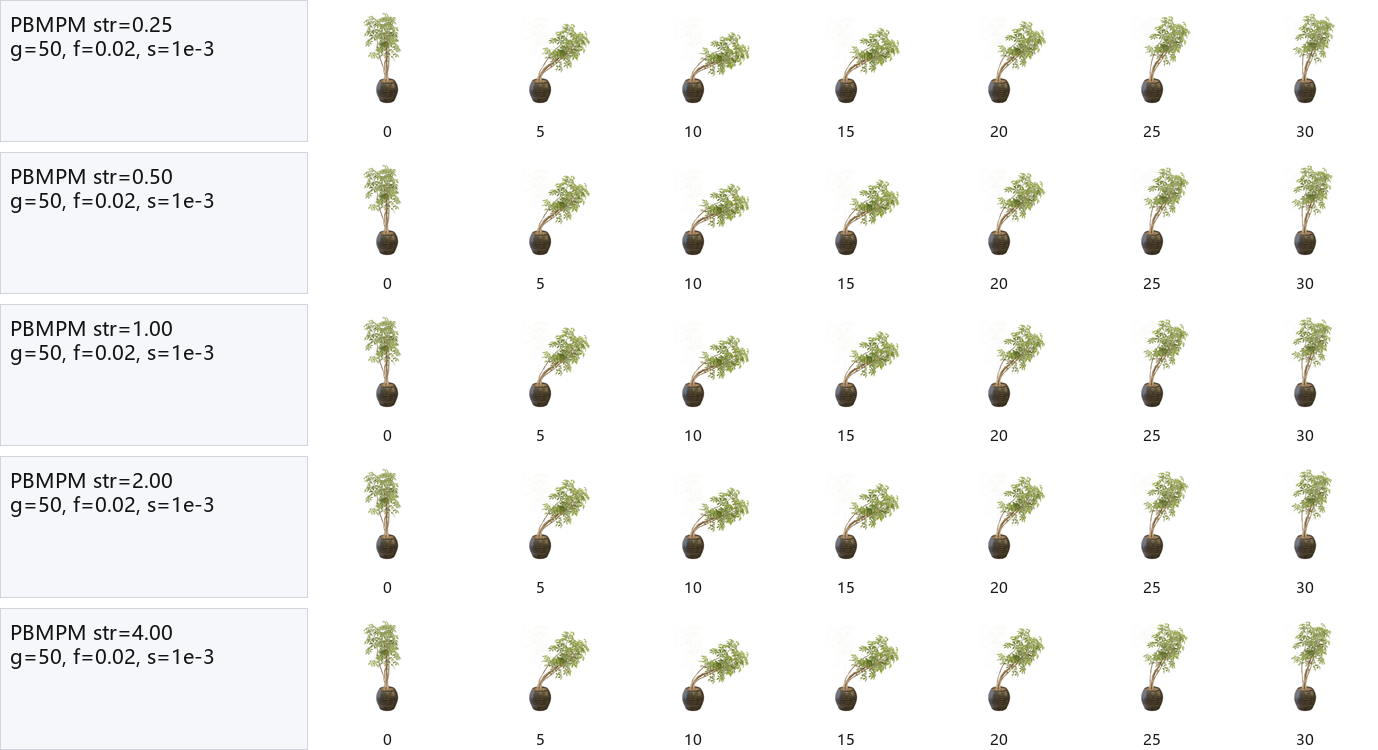
\includegraphics[width=\textwidth,height=0.45\textheight,keepaspectratio]{figures/render_strips/group_pbmpm_eval_strength_dt001.png}
    \caption{PBMPM 在 $\Delta t_{\mathrm{sub}}=10^{-3}$ 下扫描 strength 的渲染关键帧。}
    \label{fig:pbmpm-eval-strength-dt001}
\end{figure}
\FloatBarrier
在大子步设置下，strength 的边际效果有限。strength 从 $0.25$ 增至 $4.0$ 时，平均位移和 bbox 膨胀仅缓慢下降，最大位移仍约为 $1.63$，最大速度约为 $16$。这说明此时自动映射的迭代数已接近上限，主要风险来自过大的 $\Delta t_{\mathrm{sub}}$ 本身，而不是 strength 单独不足。
\begin{table}[H]
\centering
\caption{PBMPM 补充实验中的异常 run}
\label{tab:pbmpm-eval-anomaly}
\small
\resizebox{\textwidth}{!}{%
\begin{tabular}{lccccc}
\toprule
设置 & 成功 & 可用帧 & 内步/理论 & 失败原因 & $r_{\mathrm{bbox}}$ \\
\midrule
$\Delta t_{\mathrm{sub}}=10^{-3},\ \omega=0$ & 否 & 7 & 137/600 & \texttt{exit\_code\_-6} & 2.400 \\
\bottomrule
\end{tabular}%
}
\end{table}
总体而言，PBMPM 的参数评价不能只看 success 或耗时。relaxation 是高风险设置中的关键参数，解耦后可以改善 $n_{\mathrm{grid}}=100$ 和 $\Delta t_{\mathrm{sub}}=10^{-3}$ 的表现；strength 在细网格下有效，在大子步下效果有限。实际使用时仍需同时检查 displacement、velocity、acceleration、bbox 和视觉渲染结果。
